\begin{appendices}

\chapter{42TestIncrementer Example \label{incrementerExample}}

\begin{figure}[h]
\begin{42listing}
reuse L42.is/AdamTowel02
A: {
	class method incr(Num that) (return that + 1Num)
	class method str(S that) (return that + S"bar")
}
B: {
	Debug(A.incr(1Num))
	Debug(A.str(S"foo"))
	return ExitCode.normal()
}
\end{42listing}
\caption{A 42 program that is a good candidate for the 42TestIncrementer \label{42incr}}
\end{figure}

\begin{figure}[h]
\begin{42listing}
reuse L42.is/AdamTowel02
A: {
	class method incr(Num that) (return that + 1Num)
	class method str(S that) (return that + S"bar")
}

B: {
	Debug(A.incr(13Num))
	Debug(A.str(S"fooTWo"))
	return ExitCode.normal()
}
\end{42listing}
\caption{The 42 program from Figure \ref{42incr} that has been run through the 42TestIncrementer \label{incered}}
\end{figure}


\chapter{Sample bug report}

\textbf{VectorBlankVariable.L42}

\begin{42listing}
	reuse L42.is/AdemTowel02
	CacheAdamTowel02:Load.cacheTowel()

	Nums : Collections.vector(of: Num)
	Main: {
		Nums arr = Nums[_;_;_]
	}
\end{42listing}

~\\
\textbf{Expected behaviour}: Some sort of 42 error stating that variable "\_" is not in scope or cannot be found.

~\\
\textbf{Actual behaviour}: java.lang.NullPointerException
~\\
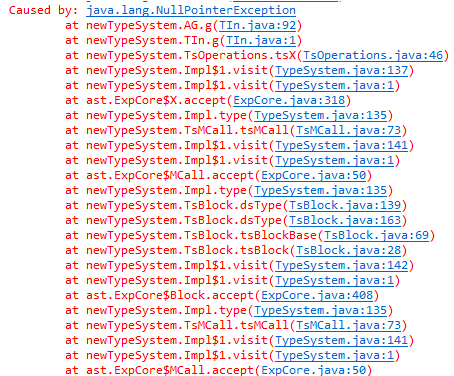
\includegraphics{bugReport}

\end{appendices}